\chapter{Results}
This chapter begins by presenting some of the central questions mentioned in the introduction. It continues with giving a general overview of the experimental results, before examining the findings in more detail. Finally the discoveries are summarized and some limitations of the experiment are highlighted.

\section{Goals}
We study how the extension of KG affects rule mining, and the role of extension methods in the process. Some central questions here are:
\begin{enumerate}
    \item Does adding new plausible facts lead to new rules being mined? 
    \item How does the PCA confidence of these rules compare to the rules mined from the original KG?
    \item Can the rules mined from the original KG also be mined after the KG is extended?
\end{enumerate}
Regarding extension methods we looked at three parameters:
\begin{itemize}
    \item the \textit{entity selection strategy} for candidate generation
    \item the \textit{KG embedding model architecture} for ranking candidates
    \item the \textit{rank cutoff value} for admitting candidates to the KG
\end{itemize}
and their role in the quantity and PCA confidence of the rules that are mined.

\section{Overview of results}
This section gives a brief overview of the results and focuses on the fact that the KG embedding choice has a considerable influence on the number of rules being mined. The majority of rules were mined from TransE-extended KGs, and were rules that upon inspection had little meaning to them. As speculated in section \ref{selected_KG_embedding_models}, the findings show that the TransE model was not a success, and this section justifies why results from this model are omitted in some later parts of the data analysis.

\subsection{KG extension sizes}
In the KG extension process there are 48 \footnote{4 (KG embedding models) $\times$ 4 (entity selection methods) $\times$ 3 (rank cutoff) = 48 parameter combinations.} different parameter combinations. This means that there are 48 different KG extensions for each original KG. Extension set sizes range from approximately 800 to 33500 triples, where the RandomBaseline model admitted the most candidates. This makes sense, as the models assign a random score to facts, so that many more receive a high rank. The \textit{trained} models give most candidates a low score because most triples usually are bad candidates. Note that the extension sizes were about the same for both datasets, while WN18RR and the family KG respectively have 88 227 and 258 235 facts, therefore the extensions for WN18RR are relatively larger than for the family KG. See figure \ref{model_extensions_boxplot} for the distribution of KG extension sizes over the KG embedding models used.

\subsection{Rule set sizes and mean PCA confidence}
\label{TransE_sucks} 
Upon examining the number of rules mined per KG extension one immediately sees some startling results, displayed clearly in figure \ref{total_rules_KG_embedding_dist}. Most rule sets do not differ drastically in size, apart from those where TransE was used, where these rule sets are \textit{exceptionally} larger. See \cref{all_sets} for a more detailed overview of the results for all KG extensions. When looking at the mean PCA confidence of the rules sets one also notes that the score for the TransE sets are mostly around 0.1, while the remaining rule sets have a score on average around 0.5.

\begin{figure}[htbp]
\centering
\begin{subfigure}{.5\textwidth}
  \centering
  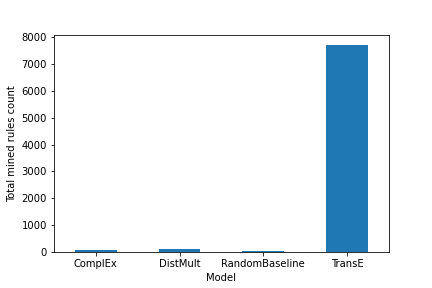
\includegraphics[width=1\linewidth]{figures/results/Total_mined_rules-model-wn18rr.png}
  \caption{WN18RR}
  \label{total_rules_KG_embedding_dist_WN18RR}
\end{subfigure}%
\begin{subfigure}{.5\textwidth}
  \centering
  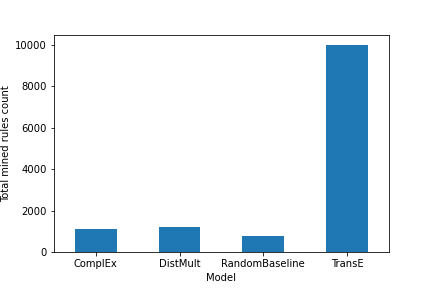
\includegraphics[width=1\linewidth]{figures/results/Total_mined_rules-model-family.png}
  \caption{Family KG}
  \label{total_rules_KG_embedding_dist_family}
\end{subfigure}
\caption[Number of total mined rules over embedding models]{Distribution of total number of mined rules over different embedding models, so the sum of all rules mined over the different KG extensions partitioned by the embedding models used.}
\label{total_rules_KG_embedding_dist}
\end{figure}

As discussed in Section \ref{TransE_peaked_in_2013} TransE is not able to learn certain relation qualities, and upon further inspection of the embedding vectors for relations in TransE the vector values all tend toward zero (see \ref{TransE_embedding_family} and \ref{TransE_embedding_WN18RR}). This can partially be explained by TransE's tendency to push the embeddings of symmetric relations toward the zero vector and its lack of ability to effectively embed complex relations. Both issues explained in section \ref{KG_embeddings_section}. It seems that while scoring decently on the performance metrics during model selection, TransE has not properly embedded the relations in the KG. 

Interestingly, the number of rules mined from TransE-extended KGs is not proportional to the number of triples added to the original KG, which is much lower relatively speaking. There is something \textit{particular} about the triples that TransE ranks highly, resulting in the introduction of more patterns in the dataset. If we look at the mentioned weaknesses of the TransE embedding model we can reach some plausible explanations.

\begin{figure}[htb]
\centering
\begin{subfigure}{.5\textwidth}
  \centering
  \includesvg[width=1\linewidth]{figures/results/wenn_wn18rr.svg}
  \caption{WN18RR KG.}
  \label{venn_wn18rr}
\end{subfigure}%
\begin{subfigure}{.5\textwidth}
  \centering
  \includesvg[width=1\linewidth]{figures/results/wenn_family.svg}
  \caption{Family KG.}
  \label{venn_family}
\end{subfigure}
\caption[New rules grouped by KGEs]{Distribution of new rules grouped according to which KGE was used to created the extended KG from which the rule was mined. Duplicates are removed.}
\label{venn}
\end{figure}

To illustrate this, let us again consider the KG from example \ref{mini_simple_KG_rules}, in which \texttt{Carol} has children \texttt{Ann} and \texttt{Bob}, and \texttt{Ann} and \texttt{Bob} are explicitly stated to be each others siblings. Due to TransE's problems regarding the embedding of complex relations \cite{transH, transR}, \texttt{Ann} and \texttt{Bob} are likely to be identically represented in the embedding space. According to the results, each relation in the family KG is represented as a null-vector in the TransE embedding. Thus all relations are considered essentially equivalent to each other. Hence, we find ourselves in a situation where \texttt{Ann} and \texttt{Bob} are equivalent, and all relations are equivalent. With these assumptions, meaningless triples such as
\texttt{(Carol, has\_spouse, Ann)}, \texttt{(Carol, has\_spouse, Bob)} and \texttt{(Bob, has\_child, Ann)} would score highly according to our TransE model. TransE will assign a high score to all original triples with the relation swapped for another. This would lead to more triples sharing common entities, resulting in more patterns arising in the data. Therefore any combination of relations in the body and consequent would gain some degree of support in the extended KG, and hence be mined with AMIE3. The meaningless triples mentioned above are simply existing triples in the example KG with the relation switched for another that is by the model considered equivalent. 

Some resulting nonsense rules from TransE extensions are shown in listing \ref{TransE_nonsense_rules}. Many of these would make sense if the relations were swapped for another, for example if \textit{relative} in the body of rule 3 were swapped with \textit{sibling} the rule would make perfect sense. The second nonsense rule in the listing, $mother(x, y) \Rightarrow child(x, y)$, was also found by DistMult. This makes sense, because for DistMult the two triples \texttt{(a, mother, b)} and \texttt{(b, mother, a)} will have the same score for all entities \texttt{a} and \texttt{b}, and the rule $mother(y, x) \Rightarrow child(x, y)$ is likely to have considerable support in the dataset. The remaining rules in listing \ref{TransE_nonsense_rules} were only found in TransE-extended KGs.

\begin{lstlisting}[mathescape=true, float, caption={Selection of nonsense rules mined from KGs extended with TransE.},captionpos=b, label={TransE_nonsense_rules}]
$spouse(x, y)  \Rightarrow father(x, y)$
$mother(x, y)   \Rightarrow child(x, y)$
$relative(y, x) \Rightarrow sibling(x, y)$
$spouse(x, y) \Rightarrow child(x,y)$
$relative(x, y) \Rightarrow sibling(x, y)$
$relative(x, z) \wedge sibling(z, y) \Rightarrow mother(x, y)$
$child(z, x) \wedge mother(z,y) \Rightarrow spouse(x, y)$
$relative(y, x) \wedge sibling(y, x) \Rightarrow father(x, y)$
$mother(z, y) \wedge mother(x, z) \Rightarrow child(x, y)$
$sibling(y, x) \wedge spouse(x, y) \Rightarrow father(x, y)$
\end{lstlisting}

Of the rules mined, 97\% (WN18RR) and 76\% (family KG) originate from KGs extended using TransE. The large number of rules produced marginalize those mined using other embedding models. Due to this and the fact that the trained TransE model has poor relational embeddings, we include rules mined from KGs extended with TransE only when examining embedding models, but not when looking at entity selection methods or rank cutoff values.






\section{Effect of parameters}
In this section we will examine the effects of each of the three main parameters in the KG extension process. Note that when looking at rules with a certain parameter the sets of rules will be a concatenation of all cases where that parameter was used. For example, if we look at the rules mined with ComplEx as the KG embedding model, then this group contains rules mined from 12 different KG extensions because we need to look at all the combinations of entity selection methods and rank cutoff values ($4\times3=12$). This is differentiated from the case where we look at rules mined from a single extended KG, which we do in \cref{Rule_comparison}.

\begin{figure}[htbp]
\centering
\begin{subfigure}{1\textwidth}
  \centering
  \includesvg[inkscapelatex=false,width=0.9\textwidth,keepaspectratio]{figures/results/rule_dist_models_hbar_family.svg}
  \caption{Family KG}
  \label{rule_dist_models_hbar_family}
\end{subfigure}%
\hfill
\begin{subfigure}{1\textwidth}
  \centering
  \includesvg[inkscapelatex=false,width=0.9\textwidth,keepaspectratio]{figures/results/rule_dist_models_hbar_wn18rr.svg}
  \caption{WN18RR KG}
  \label{rule_dist_models_hbar_wn18rr}
\end{subfigure}
\caption[Rules and their types over KG embedding models]{Distribution of rules over KG embedding models, not counting duplicate rules that were mined from multiple KGs. Note that the bar for TransE extends far beyond the chart, so the unusually high number of different rules mined from TransE extensions is not properly shown here. The single original rule not found by DistMult in the family KG is $child(x, y) \Rightarrow mother(y,x)$. This rule has the second lowest PCA confidence of all the original family KG rules.}
\label{rule_dist_models_hbar}
\end{figure}

\subsection{Effect of KG embedding model}
At the first glance of the boxplots in figure \ref{fig:PCA_models_boxplot} it may seem odd that the PCA confidence of rules mined from RandomBaseline extensions is so high. Boxplots are used to represent the spread of data through their quartlies \cite{dutoit2012graphical}. The box itself covers $Q_1-Q_3$, with the horizontal line in the box marking the median. The median PCA confidence for the original rules is indicated by the dashed line across the plots. The boxplots used in this thesis also have \textit{whiskers}, which are the lines extending vertically out of the box. Whiskers give an indication of the variability of the data outside the upper and lower quartiles (respectively $Q_1$ and $Q_3$). Points beyond the whiskers are considered outliers.

\begin{figure}[htbp]
\centering
\begin{subfigure}{.5\textwidth}
  \centering
  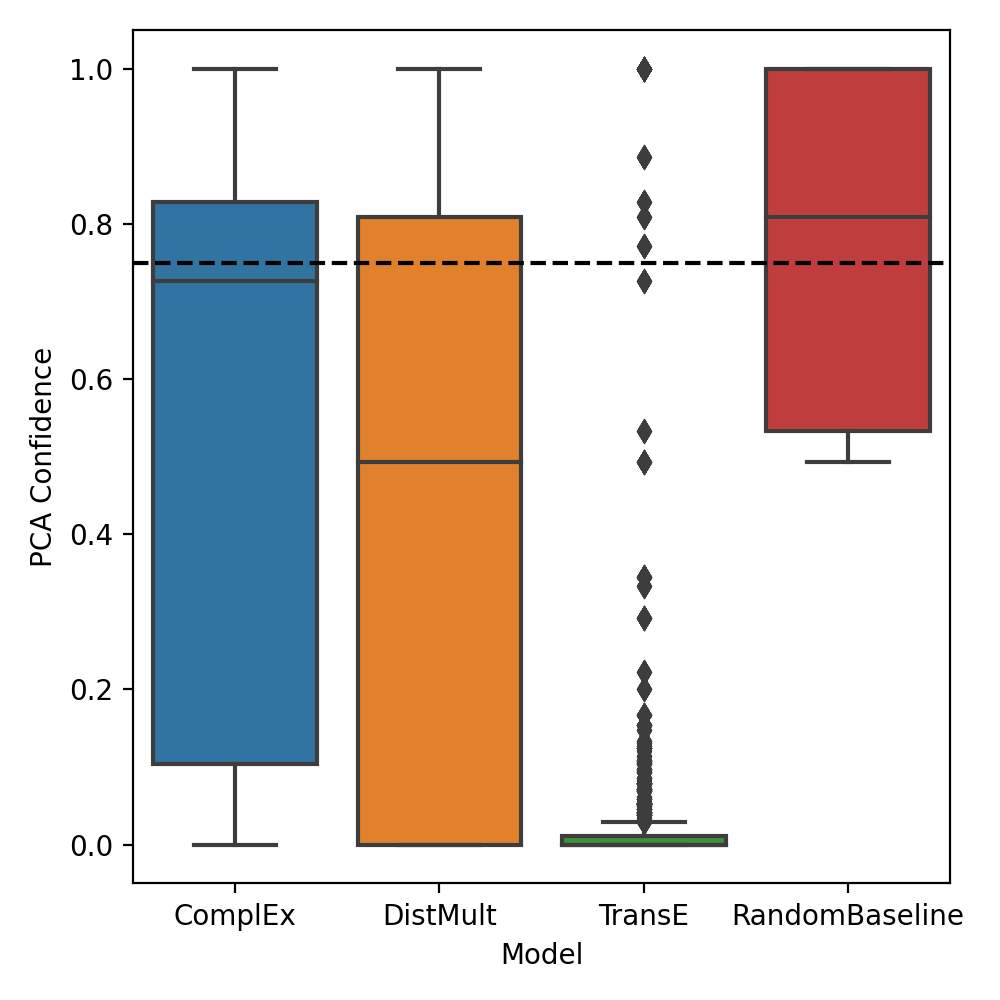
\includegraphics[width=1\linewidth]{figures/results/PCA_models/PCA-models_wn18rr.png}
  \caption{Original WN18RR KG}
  \label{fig:PCA-models_wn18rr_boxplot_sub}
\end{subfigure}%
\begin{subfigure}{.5\textwidth}
  \centering
  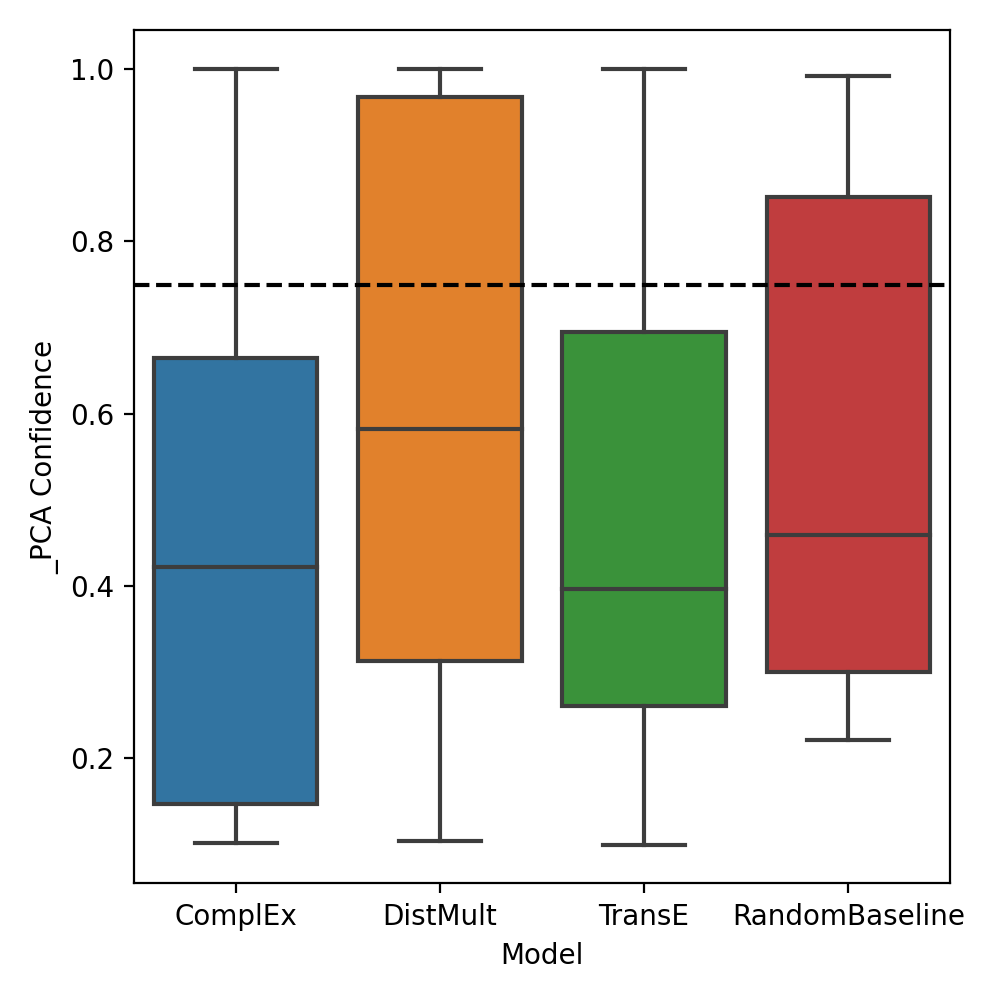
\includegraphics[width=1\linewidth]{figures/results/PCA_models/_PCA-models_wn18rr.png}
  \caption{Extended WN18RR KG}
  \label{fig:_PCA_models_wn18rr_boxplot_sub}
\end{subfigure}
\begin{subfigure}{.5\textwidth}
  \centering
  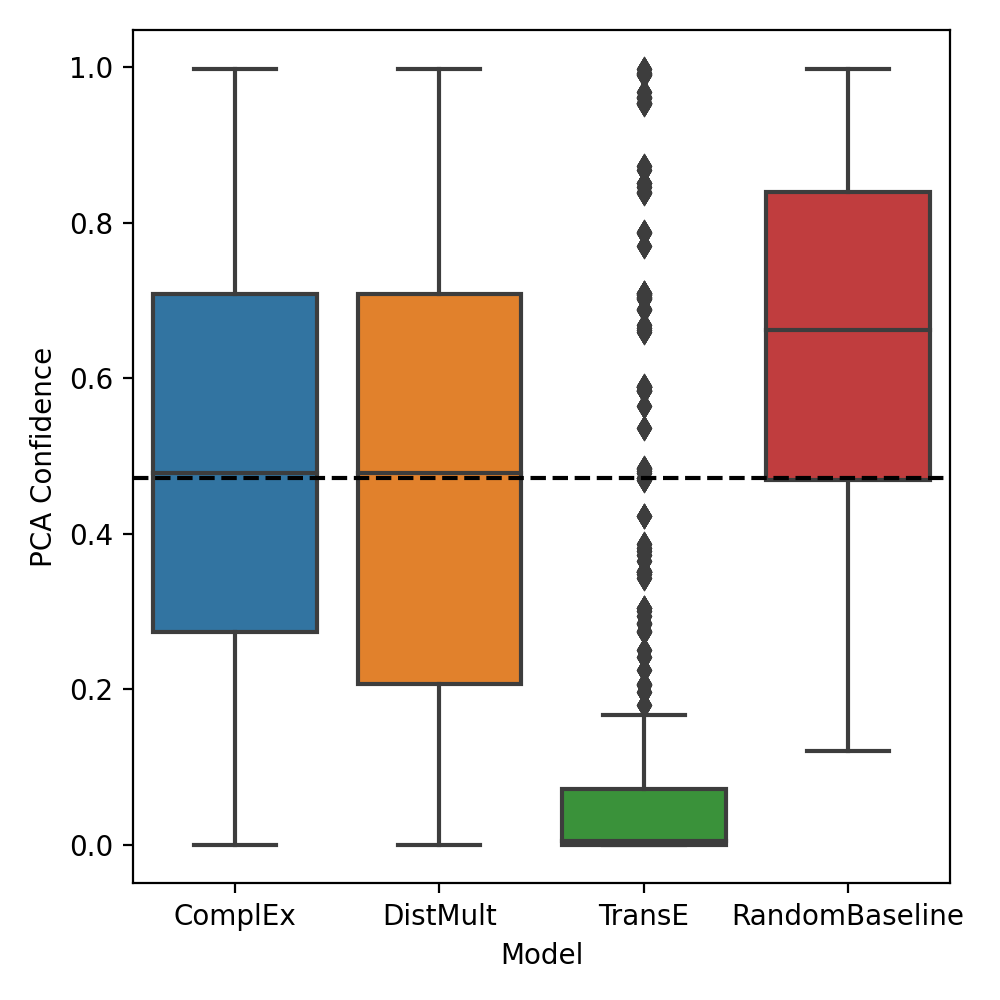
\includegraphics[width=1\linewidth]{figures/results/PCA_models/PCA-models_family.png}
  \caption{Original family KG}
  \label{fig:models_family_boxplot_sub}
\end{subfigure}%
\begin{subfigure}{.5\textwidth}
  \centering
  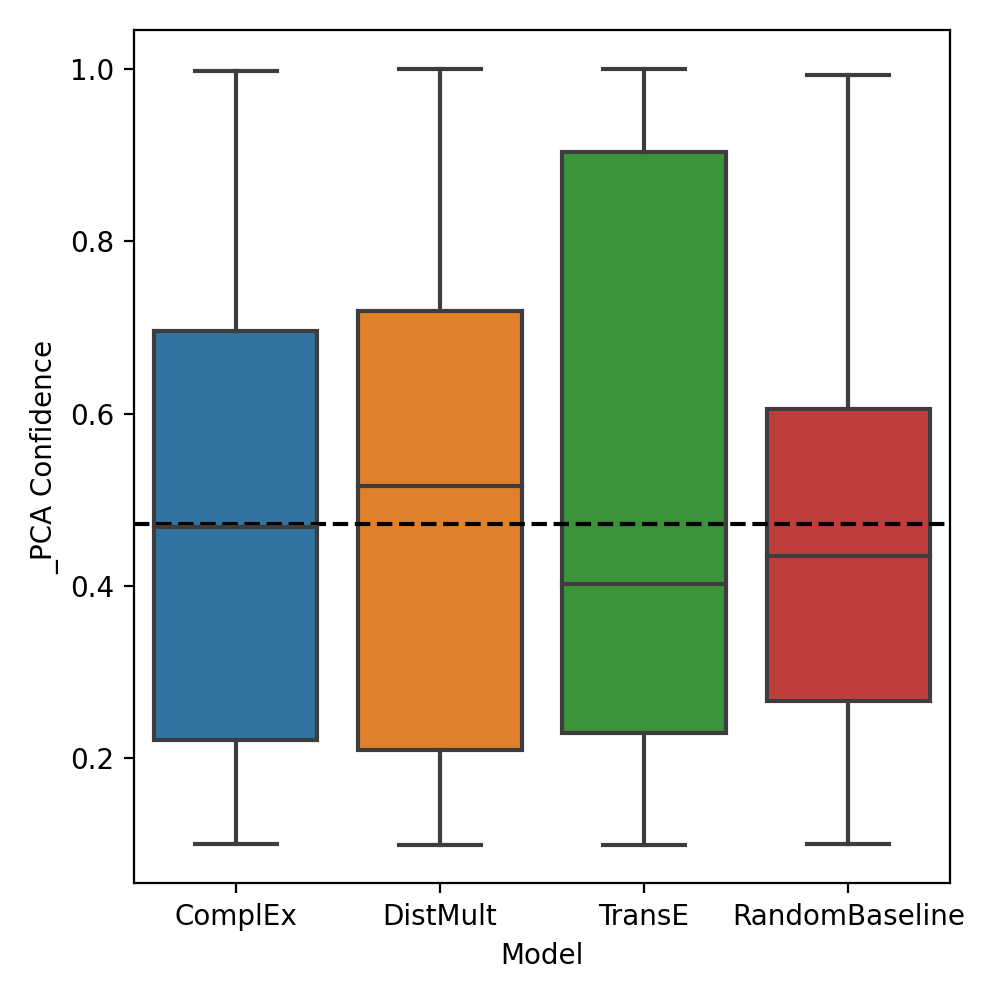
\includegraphics[width=1\linewidth]{figures/results/PCA_models/_PCA-models_family.png}
  \caption{Extended family KG}
  \label{fig:_PCA_models_family_boxplot_sub}
\end{subfigure}
\caption[Dist. of PCA conf. rules by KG embedding models]{Distribution of PCA confidence of mined rules by KG embedding models. PCA confidence scores are calculated on the original KG (\ref{fig:PCA-models_wn18rr_boxplot_sub}, \ref{fig:models_family_boxplot_sub}) and the extended KG from which the rules are mined (\ref{fig:_PCA_models_wn18rr_boxplot_sub}, \ref{fig:_PCA_models_family_boxplot_sub}). A rule can be mined from multiple KGs, therefore this graph shows duplicates. The dashed line represents the median PCA confidence of the rules mined from the original KG.}
\label{fig:PCA_models_boxplot}
\end{figure}

By looking at figure \ref{rule_dist_models_hbar} it becomes apparent that there are few different rules mined from the RandomBaseline extensions. In the WN18RR case no new rules were found, and a single original rule was also never mined. The omitted rule,
\[ has\_part(x, z) \wedge hypernym(y, z) \Rightarrow has\_part(x, y)\]
has the lowest PCA confidence out of all the original rules. Since there already was little support in the KG for the rule, the addition of noise may have obscured too much evidence for the algorithm to consider the rule significant. See table \ref{original_rules_found_by_baseline_WN18RR} to see all rules mined from the original WN18RR KG, sorted by their PCA confidence.
% check RandomBaseline_original_rules.ipynb to see if there is a new rule.

\begin{table}[htp]
\centering
\begin{tabular}{l|cc|cc|cc}
\multicolumn{1}{c}{\multirow{2}{*}{\textbf{Model}}} & \multicolumn{2}{c}{\textbf{Original rules}} & \multicolumn{2}{c}{\textbf{New rules}} & \multicolumn{2}{c}{\textbf{Orig. not found}}         \\
\multicolumn{1}{c}{}                                & Count    & \% of mined    & Count  & \% of mined & Count & \multicolumn{1}{c}\% of original \\ \hline
Baseline                                            & 85             & 100\%                      & 0            & 0\%                     & 9           & 10\%                                           \\
TransE                                              & 94             & 9\%                        & 986          & 91\%                    & 0           & 0\%                                            \\
DistMult                                            & 93             & 51\%                       & 90           & 49\%                    & 1           & 1\%                                            \\
ComplEx                                             & 94             & 69\%                       & 43           & 31\%                    & 0           & 0\%                                           
\end{tabular}
\caption[Dist. rules over KG embedding models - family KG.]{Distribution of all the rules mined over KG embedding models. KG: family KG.}
\label{Tab:table_rules_models_family}
\end{table}

\begin{table}[htp]
\centering
\begin{tabular}{l|cc|cc|cc}
\multicolumn{1}{c}{\multirow{2}{*}{\textbf{Model}}} & \multicolumn{2}{c}{\textbf{Original rules}} & \multicolumn{2}{c}{\textbf{New rules}} & \multicolumn{2}{c}{\textbf{Orig. not found}}         \\
\multicolumn{1}{c}{}                                & Count    & \% of mined    & Count  & \% of mined & Count & \multicolumn{1}{c}\% of original \\ \hline
Baseline                                            & 9             & 100\%                      & 0            & 0\%                     & 1           & 10\%                                           \\
TransE                                              & 10             & 1\%                        & 659          & 99\%                    & 0           & 0\%                                            \\
DistMult                                            & 10             & 67\%                       & 5           & 33\%                    & 0           & 0\%                                            \\
ComplEx                                             & 10             & 59\%                       & 7           & 41\%                    & 0           & 0\%                                           
\end{tabular}
\caption[Dist. rules over KG embedding models - WN18RR KG.]{Distribution of all the rules mined over KG embedding models. KG: WN18RR.}
\label{Tab:table_rules_models_wn18rr}
\end{table}

The family KG produced similar results, where AMIE3 failed to find 9 original rules in the RandomBaseline-extended KGs. All of these rules were among those with the lowest PCA confidence of the original rules. Refer to table \ref{original_rules_found_by_baseline_WN18RR} for all rules mined from the original family KG, sorted by their PCA confidence. When the rules with lowest PCA condifence in a set are removed, then the median PCA confidence naturally goes up. This explains how the RandomBaseline rules have a higher median PCA confidence than the original, shown in tables \ref{Tab:table_rules_models_family} and \ref{Tab:table_rules_models_wn18rr}.

As presented in \cref{TransE_sucks}, AMIE3 mines a great deal more rules from KGs extended with TransE. Due to the low mean PCA confidence for these rules (0.038 for WN18RR and 0.089 for the family KG) it is clear that there is little support for the rules in the original KGs. If one however evaluates the TransE rules on the \textit{extended} KGs they were mined from, the PCA confidence increases substantially, as seen in figures \ref{fig:_PCA_models_wn18rr_boxplot_sub} and \ref{fig:_PCA_models_family_boxplot_sub}. So even though most of these rules have little support from the original KGs, it was no mistake that AMIE3 mined so many rules from the TransE-extended KGs.


DistMult and ComplEx are closely related embedding models as they have similar scoring functions (the scoring function of ComplEx corresponds to that of DistMult but with real embeddings), and perform similarly on benchmark datasets \cite{complEx}. As mentioned in \cref{TransE_peaked_in_2013}, DistMult is not able to represent asymmetric relations. Although AMIE3 can only mine Horn rules, thereby a rule defining the asymmetry of a relation cannot be mined, this may still affect the the quality of the embedding and thus the KG extension. From the results it seems that ComplEx is a somewhat stricter model, in the sense that it ranks candidate triples lower against corrupted triples than DistMult does. This is evidenced by the fact that the KG extension sizes are larger for DistMult than for ComplEx; DistMult is admitting more candidates. For example, of the candidates generated with the entity selection method "probabilistic" from the WN18RR KG, DistMult assigned 1468 candidates rank 1 while ComplEx only did this for 866 candidates. As a result, more rules are mined from DistMult-extended KGs. 

\newpage
\subsection{Effect of entity selection method}
The \textit{probabilistic}, \textit{random}, and the \textit{least frequent} entity selection strategies perform relatively similarly if we look at the PCA confidence box plots in figure \ref{fig:PCA_entity_boxplot}. The \textit{most frequent} strategy, however, performs worse, both on the WN18RR and family KG. This is consistent with AmpliGraph's assumption that the most frequent entities are less likely to have missing facts \cite{kge_tutorial}.

In the WN18RR KG all original rules were found, but in the family KG only the \textit{least frequent} strategy resulted in all the original rules being mined. It also resulted in the least new rules being mined, while the \textit{most frequent} strategy led to the most new rules.

Overall it seems like \textit{probabilistic}, \textit{random}, and the \textit{least frequent} entity selection strategies all are appropriate in regard to maintaining PCA confidence. If however the goal is to mine many new rules then \textit{most frequent} apears to be best suited, though at the sacrifice of PCA confidence.

\begin{figure}[htbp]
\centering
\begin{subfigure}{.5\textwidth}
  \centering
  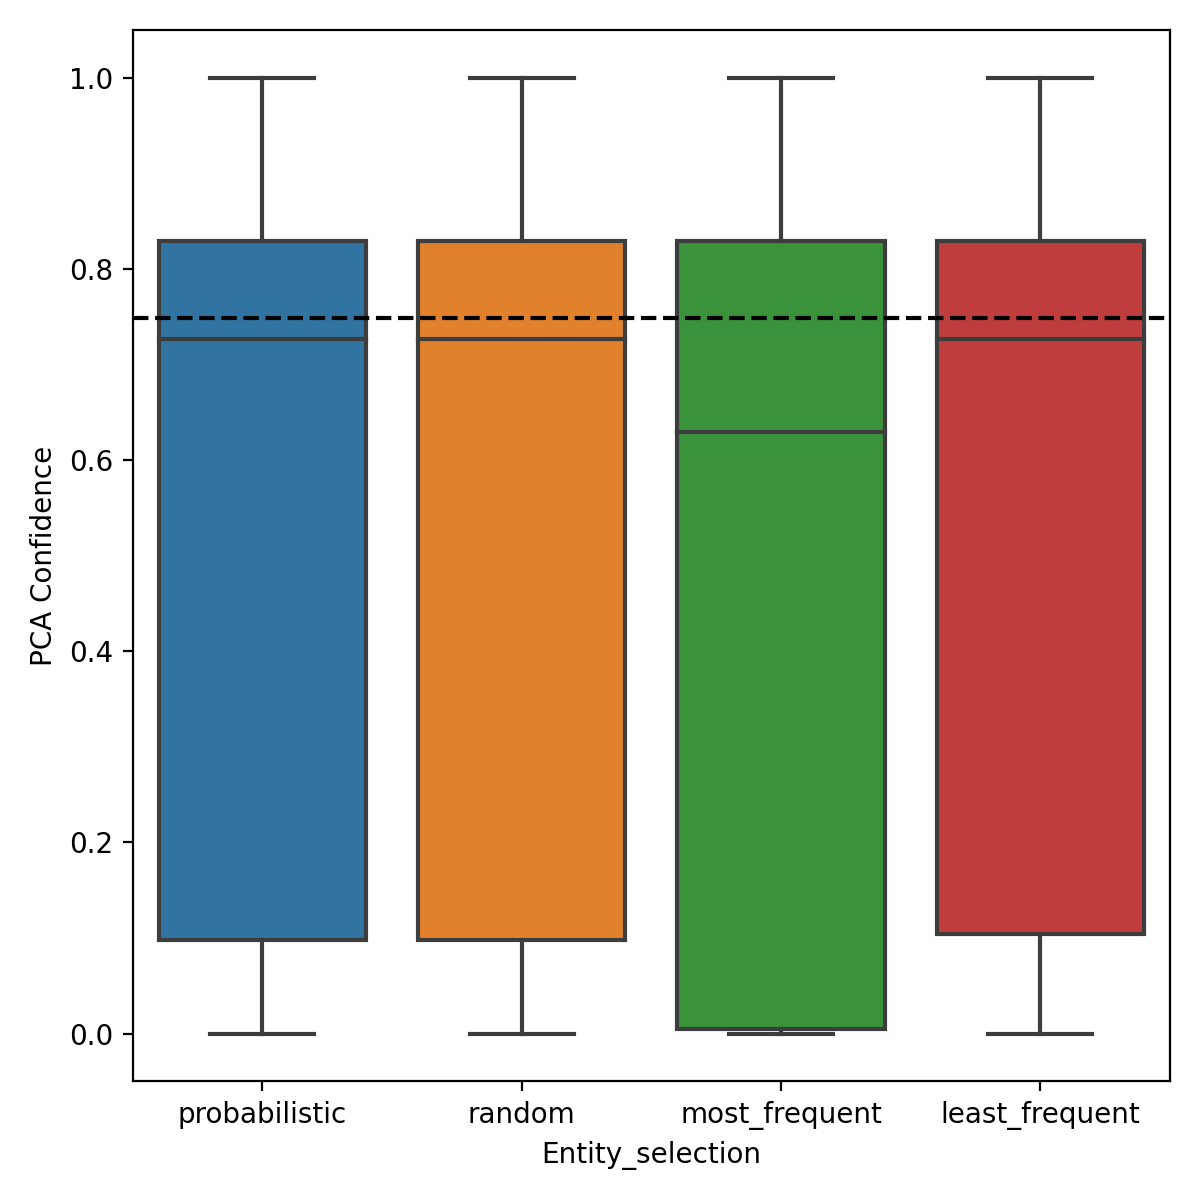
\includegraphics[width=1\linewidth]{figures/results/entity_selection/PCA-entity_wn18rr.png}
  \caption{Original WN18RR KG}
  \label{fig:PCA-entity_wn18rr_boxplot_sub}
\end{subfigure}%
\begin{subfigure}{.5\textwidth}
  \centering
  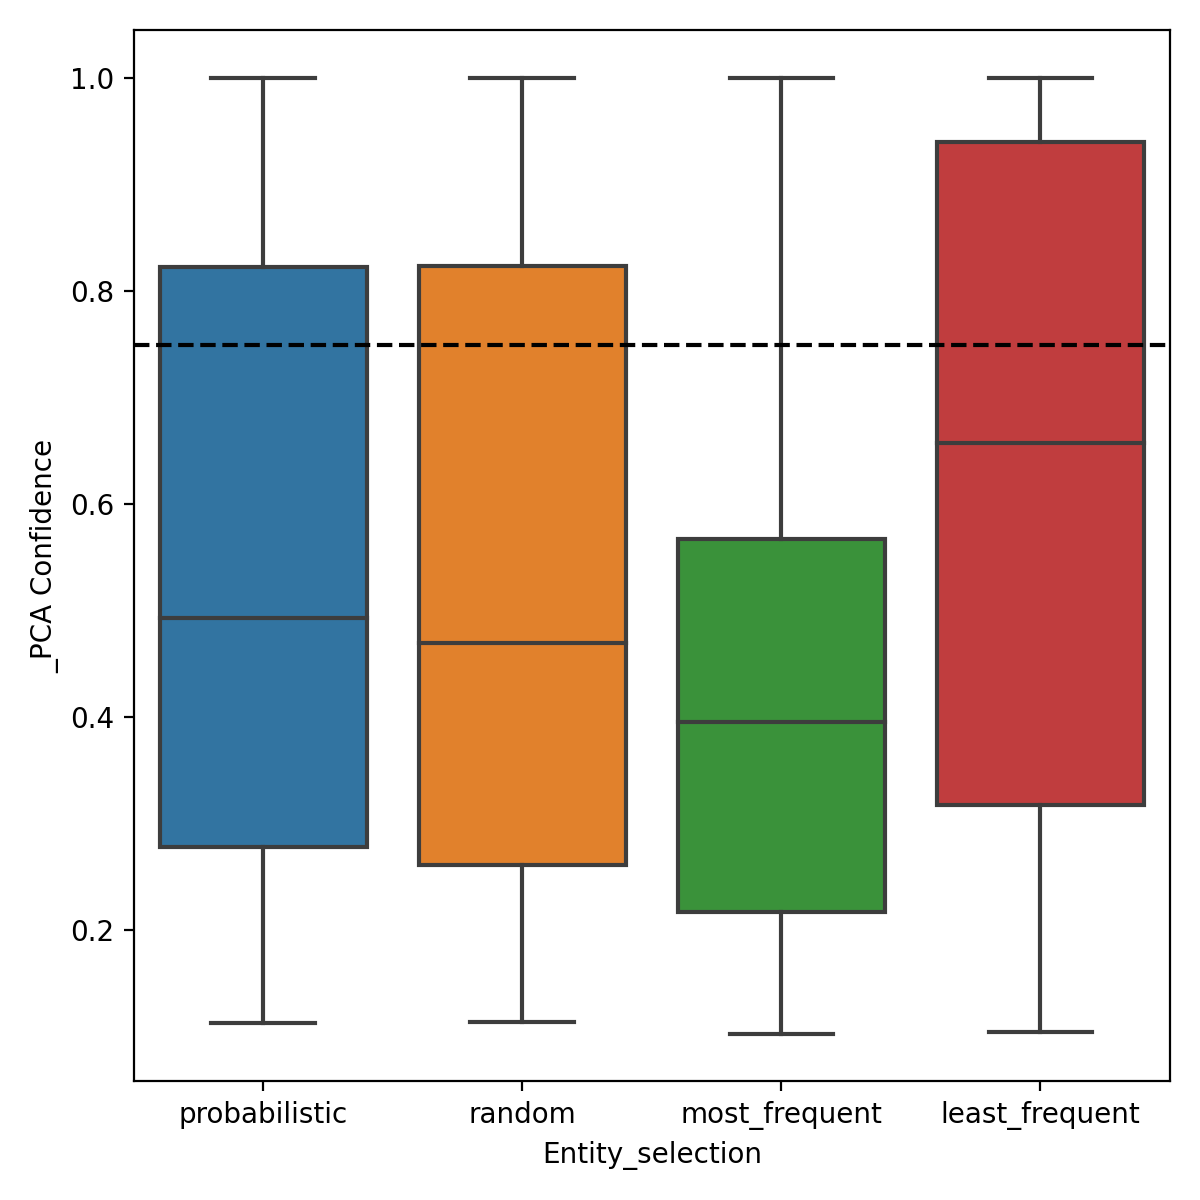
\includegraphics[width=1\linewidth]{figures/results/entity_selection/_PCA-entity_wn18rr.png}
  \caption{Extended WN18RR KG}
  \label{fig:_PCA_entity_wn18rr_boxplot_sub}
\end{subfigure}
\begin{subfigure}{.5\textwidth}
  \centering
  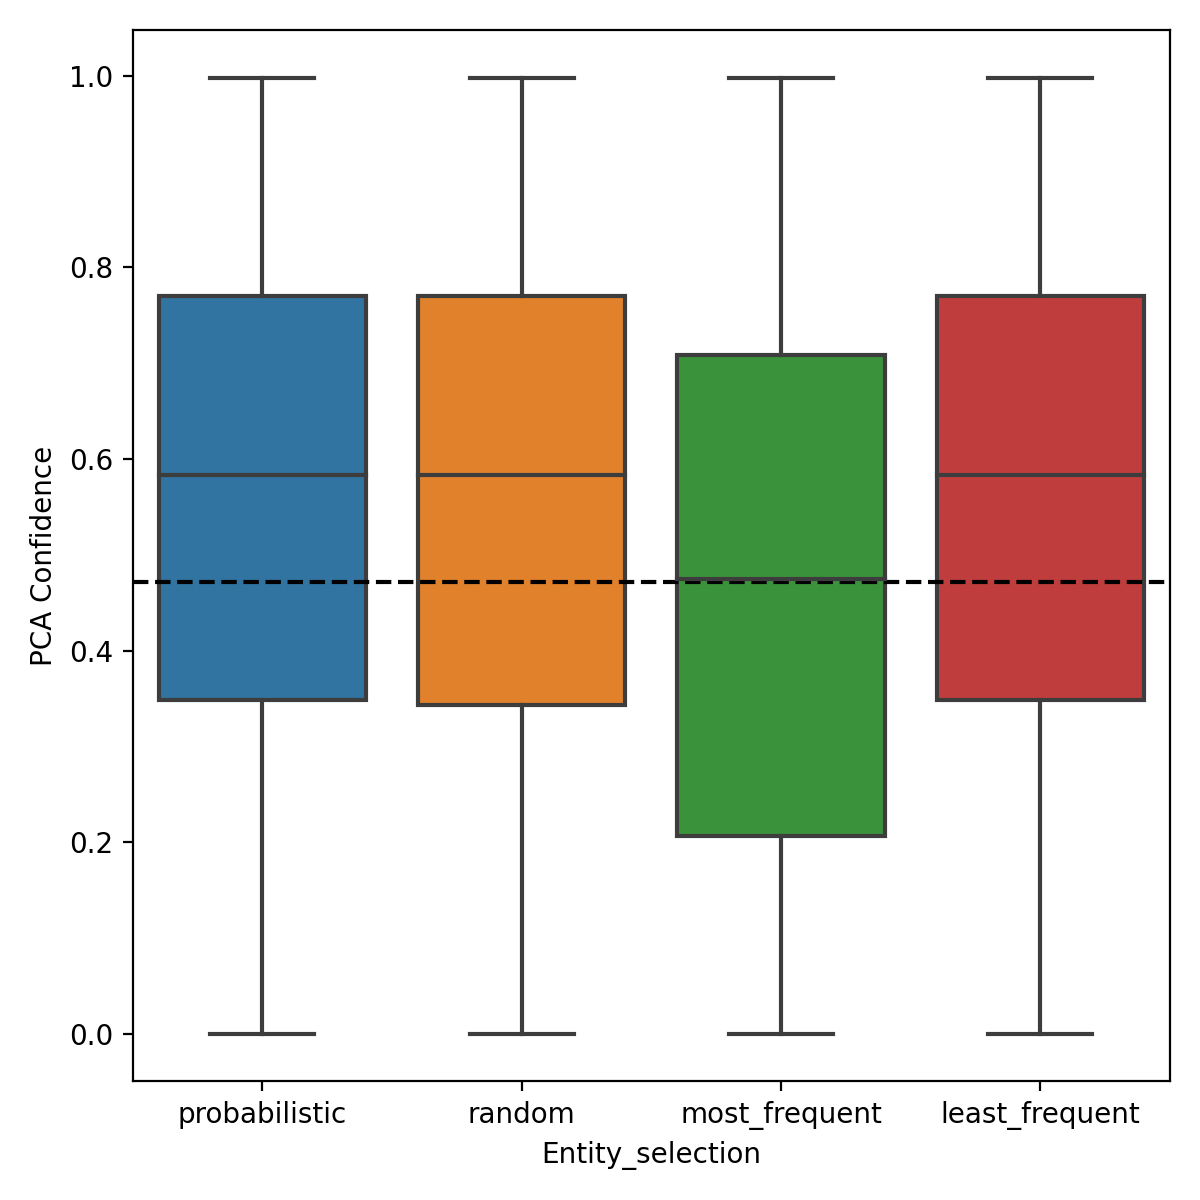
\includegraphics[width=1\linewidth]{figures/results/entity_selection/PCA-entity_family.png}
  \caption{Original family KG}
  \label{fig:models_entity_boxplot_sub}
\end{subfigure}%
\begin{subfigure}{.5\textwidth}
  \centering
  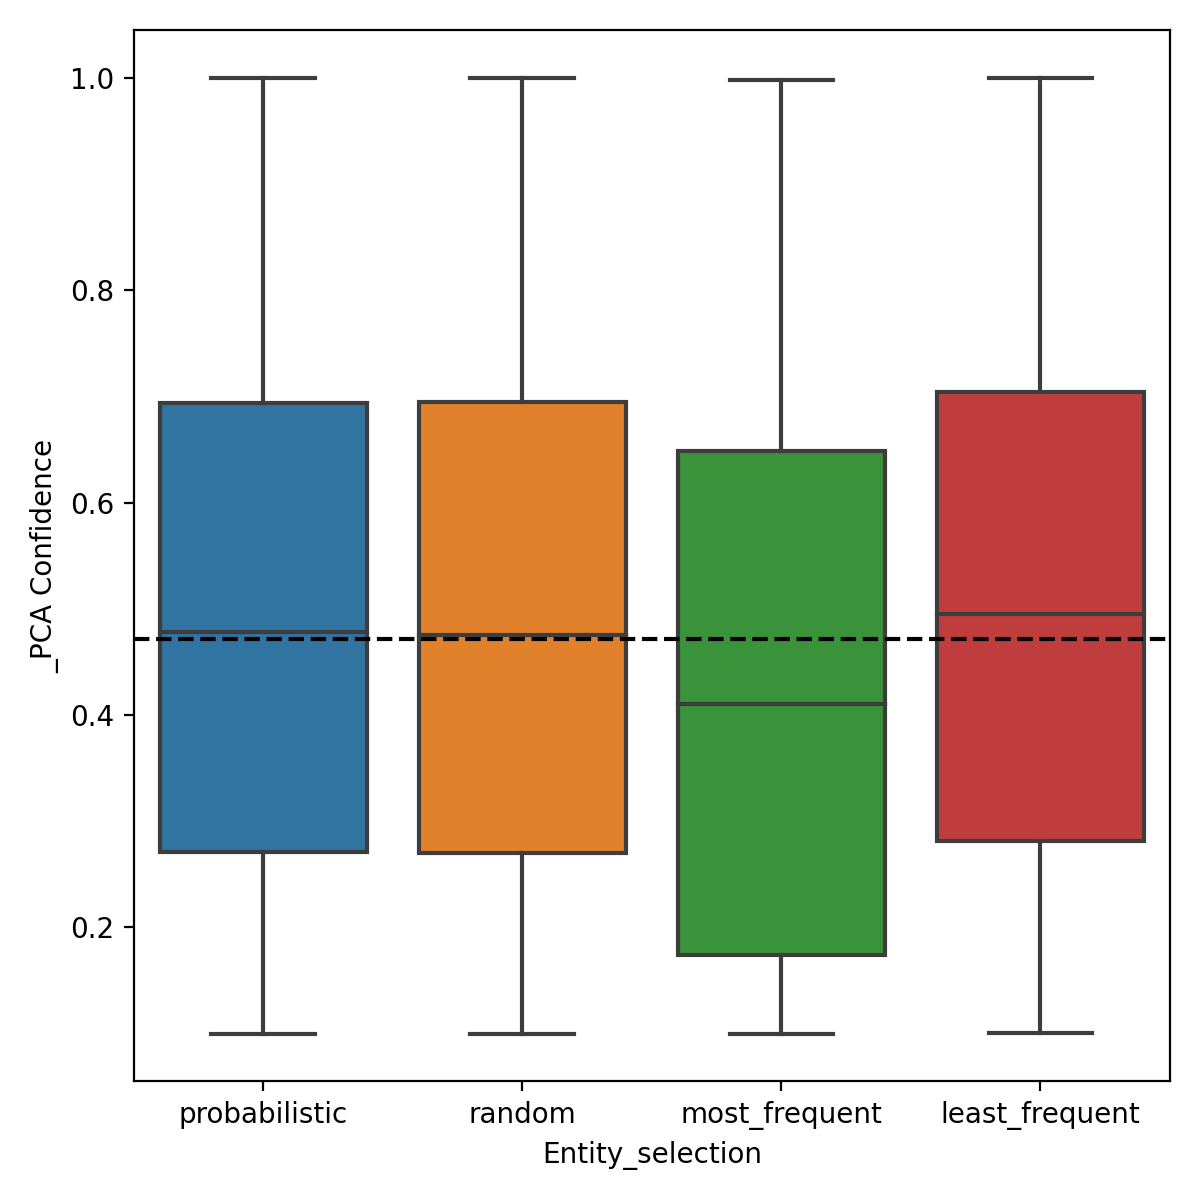
\includegraphics[width=1\linewidth]{figures/results/entity_selection/_PCA-entity_family.png}
  \caption{Extended family KG}
  \label{fig:_PCA_entity_family_boxplot_sub}
\end{subfigure}
\caption[Dist. of PCA conf. of rules by entity selection strategies]{Distribution of PCA confidence of mined rules by entity selection strategies. PCA confidence scores are calculated on the original KG (\ref{fig:PCA-entity_wn18rr_boxplot_sub}, \ref{fig:models_entity_boxplot_sub}) and the extended KG from which the rules are mined (\ref{fig:_PCA_entity_wn18rr_boxplot_sub}, \ref{fig:_PCA_entity_family_boxplot_sub}). A rule can be mined from multiple KGs, therefore this graph shows duplicates. The dashed line represents the median PCA confidence of the rules mined from the original KG.}
\label{fig:PCA_entity_boxplot}
\end{figure}

\begin{table}[htp]
\centering
\begin{tabular}{l|cc|cc|cc}
\multicolumn{1}{c}{\multirow{2}{*}{\textbf{Strategy}}} & \multicolumn{2}{c}{\textbf{Original rules}} & \multicolumn{2}{c}{\textbf{New rules}} & \multicolumn{2}{c}{\textbf{Orig. not found}}         \\
\multicolumn{1}{c}{}                                & Count    & \% of mined    & Count  & \% of mined & Count & \multicolumn{1}{c}\% of original \\ \hline
Random                                            & 90             & 71\%                      & 36            & 29\%                     & 4           & 4\%                                           \\
Most freq.                                              & 88             & 46\%                        & 105          & 54\%                    & 6           & 6\%                                            \\
Least freq                                            & 94             & 77\%                       & 28           & 33\%                    & 0           & 0\%                                            \\
Probabilistic                                             & 91             & 73\%                       & 33           & 27\%                    & 3           & 3\%                                           
\end{tabular}
\caption[Dist. of rules over entity selection strategies - family KG.]{Distribution of all the rules mined over entity selection strategies for the family KG.}
\label{Tab:table_rules_entities_family}
\end{table}

\begin{table}[htp]
\centering
\begin{tabular}{l|cc|cc|cc}
\multicolumn{1}{c}{\multirow{2}{*}{\textbf{Strategy}}} & \multicolumn{2}{c}{\textbf{Original rules}} & \multicolumn{2}{c}{\textbf{New rules}} & \multicolumn{2}{c}{\textbf{Orig. not found}}         \\
\multicolumn{1}{c}{}                                & Count    & \% of mined    & Count  & \% of mined & Count & \multicolumn{1}{c}\% of original \\ \hline
Random                                            & 10             & 53\%                      & 9            & 47\%                     & 0           & 0\%                                           \\
Most freq.                                              & 10             & 42\%                        & 14          & 58\%                    & 0           & 0\%                                            \\
Least freq.                                            & 10             & 48\%                       & 11           & 52\%                    & 0           & 0\%                                            \\
Probabilistic                                             & 10             & 45\%                       & 12           & 55\%                    & 0           & 0\%                                           
\end{tabular}
\caption[Dist. of rules over entity selection strategies - WN18RR KG.]{Distribution of all the rules mined over entity selection strategies. KG: WN18RR.}
\label{Tab:table_rules_entities_wn18rr}
\end{table}

\iffalse
\begin{figure*}[htb]
        \centering
        \begin{subfigure}[b]{0.49\textwidth}
            \centering
            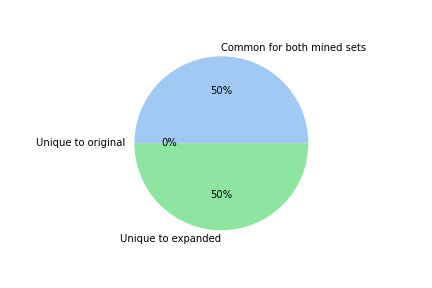
\includegraphics[width=\textwidth]{figures/results/entity_selection/pie_charts/probabilistic_wn18rr.png}
            \caption[complEx_pie]%
            {{\small Probabilistic}}    
            \label{fig:probabilistic_pie_wn18rr}
        \end{subfigure}
        \hfill
        \begin{subfigure}[b]{0.49\textwidth}  
            \centering 
            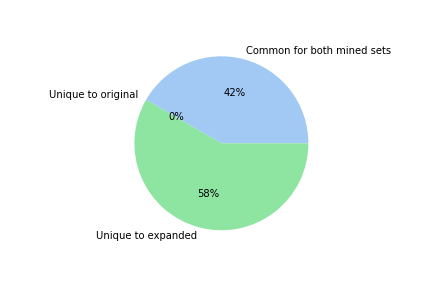
\includegraphics[width=\textwidth]{figures/results/entity_selection/pie_charts/random_wn18rr.png}
            \caption[]%
            {{\small Random}}    
            \label{random_pie_wn18rr}
        \end{subfigure}
        \vskip\baselineskip
        \begin{subfigure}[b]{0.49\textwidth}   
            \centering 
            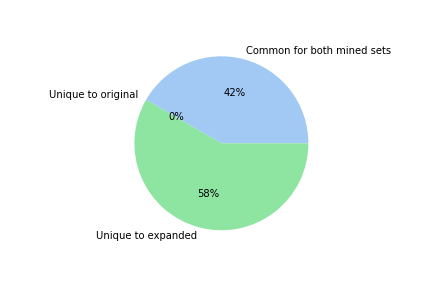
\includegraphics[width=\textwidth]{figures/results/entity_selection/pie_charts/most_frequent_wn18rr.png}
            \caption[]%
            {{\small Most Frequent}}    
            \label{fig:most_pie_wn18rr}
        \end{subfigure}
        \hfill
        \begin{subfigure}[b]{0.49\textwidth}   
            \centering 
            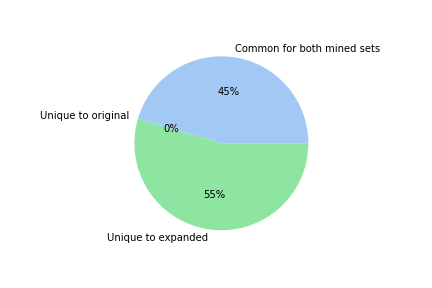
\includegraphics[width=\textwidth]{figures/results/entity_selection/pie_charts/least_frequent_wn18rr.png}
            \caption[]%
            {{\small Least Frequent}}    
            \label{fig:least_pie_wn18rr}
        \end{subfigure}
        \caption[]
        {\small Distribution of all the rules mined over entity selection strategies for WN18RR.} 
        \label{fig:entity_pies_wn18rr}
    \end{figure*}
    
    
    \begin{figure*}[htb]
        \centering
        \begin{subfigure}[b]{0.49\textwidth}
            \centering
            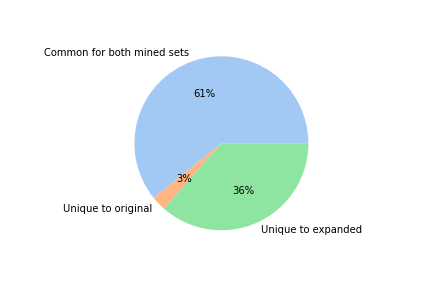
\includegraphics[width=\textwidth]{figures/results/entity_selection/pie_charts/Probabilistic_selection_family.png}
            \caption[]%
            {{\small Probabilistic}}    
            \label{fig:probablilistic_pie_family}
        \end{subfigure}
        \hfill
        \begin{subfigure}[b]{0.49\textwidth}  
            \centering 
            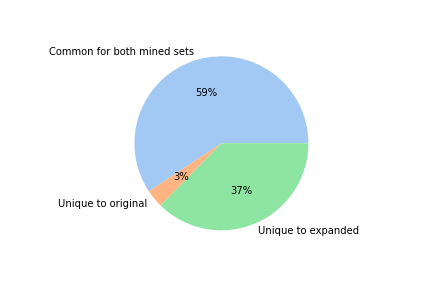
\includegraphics[width=\textwidth]{figures/results/entity_selection/pie_charts/random_family.png}
            \caption[]%
            {{\small Random}}    
            \label{fig:random_pie_family}
        \end{subfigure}
        \vskip\baselineskip
        \begin{subfigure}[b]{0.49\textwidth}   
            \centering 
            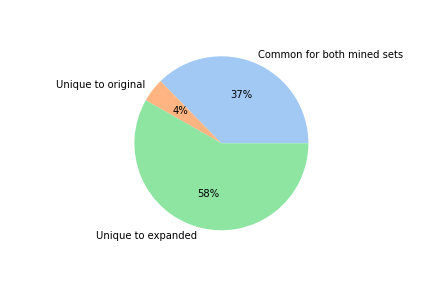
\includegraphics[width=\textwidth]{figures/results/entity_selection/pie_charts/most_frequent_family.png}
            \caption[]%
            {{\small Most Frequent}}    
            \label{fig:most_pie_family}
        \end{subfigure}
        \hfill
        \begin{subfigure}[b]{0.49\textwidth}   
            \centering 
            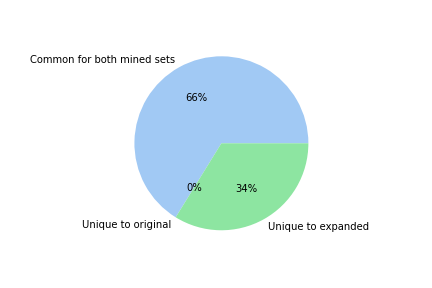
\includegraphics[width=\textwidth]{figures/results/entity_selection/pie_charts/least_frequent_family.png}
            \caption[]%
            {{\small Least Frequent}}    
            \label{fig:least_pie_family}
        \end{subfigure}
        \caption[]
        {\small Distribution of all the rules mined over entity selection strategies for the family KG.} 
        \label{fig:entity_pies_family}
    \end{figure*}

\fi




\newpage
\subsection{Effect of rank cutoff value}
Rank cutoff values determine which candidates are admitted to the KG. Only those with rank on the cutoff or above are accepted. Therefore, the lower the rank cutoff, the more candidates are added to the KG. The box plots in \cref{rank_extensions_boxplot} show evidence of this. The tables \ref{Tab:table_rules_ranks_wn18rr} and \ref{Tab:table_rules_ranks_family} both show that when the rank cutoff was 1, all the original rules were found. Decrease in rank cutoff led to the mining of more new rules, but  also led to some original rules not being mined, especially in the WN18RR case. PCA confidence-wise the rank cutoff values had a slightly different effect on the two datasets. In the WN18RR dataset there was little difference in PCA confidence over the ranks when calculated over the original KG, while for the family KG the PCA confidence was increased at rank cutoff 4 and 7, with no change at rank cutoff 1. When calculated over the KG extensions, rank 1 and 4 did worse than the mean of the original rules, while rank cutoff 7 did significantly better. On the family KG PCA confidence calculated on the extended KGs led to little variety over the rank values. Rank 1 resulted on the same median as the original rules, rank 4 just above and rank 7 just below. Overall it seems like if the goal is to find many new rules, then a higher rank cutoff values is more appropriate.

\begin{figure}[htb]
\centering
\begin{subfigure}{.5\textwidth}
  \centering
  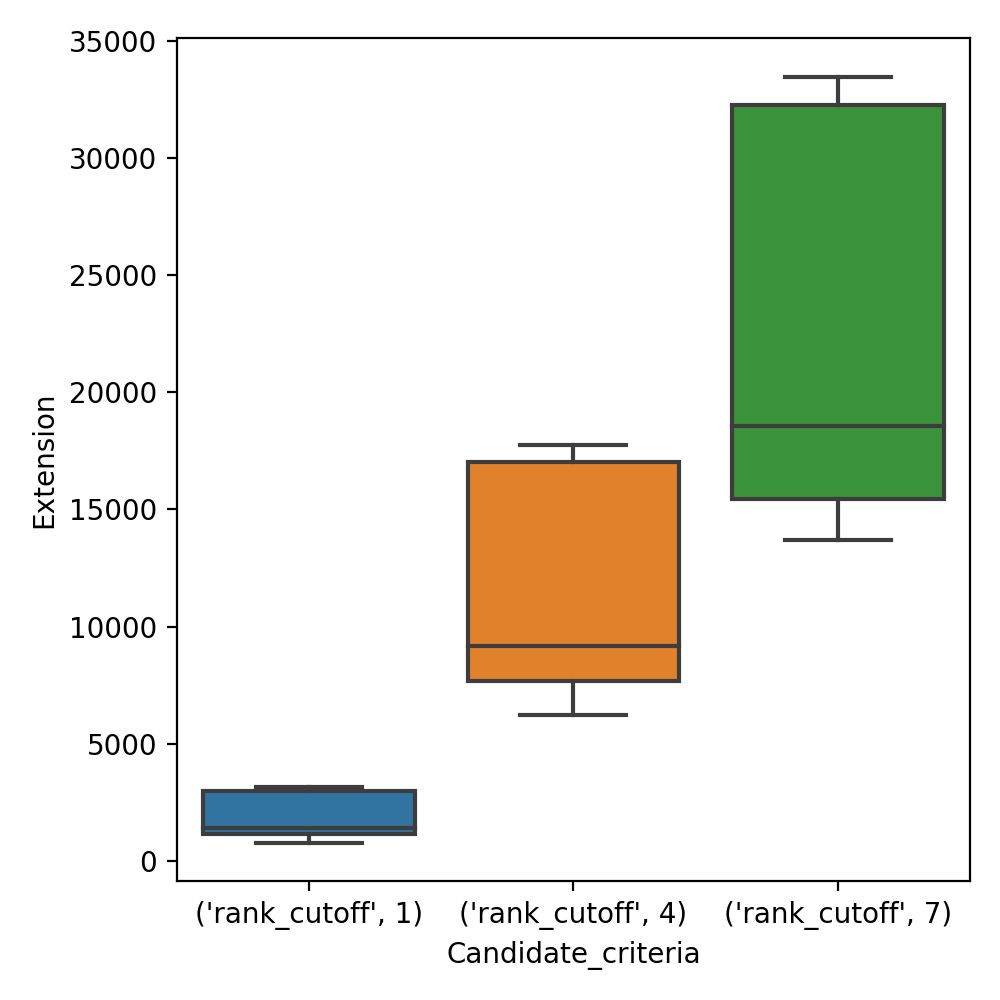
\includegraphics[width=1\linewidth]{figures/results/ranks/Extension_size_entity_wn18rr.png}
  \caption{WN18RR KG.}
  \label{fig:rank_extension_wn18rr_boxplot_sub}
\end{subfigure}%
\begin{subfigure}{.5\textwidth}
  \centering
  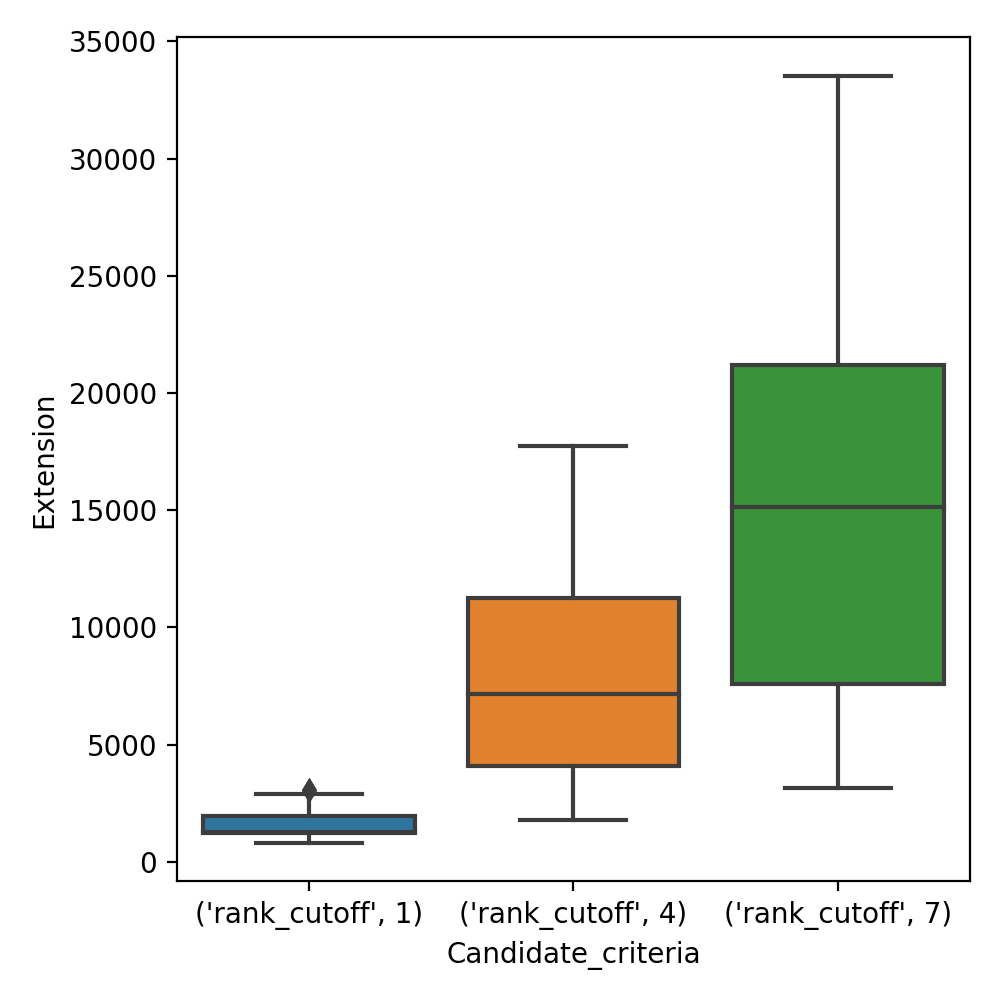
\includegraphics[width=1\linewidth]{figures/results/ranks/Extension_size_entity_family.png}
  \caption{Family KG.}
  \label{fig:rank_extension_family_boxplot_sub}
\end{subfigure}
\caption{Distribution of KG extension sizes over rank cutoff values.}
\label{rank_extensions_boxplot}
\end{figure}

\begin{figure}[!htb]
\centering
\begin{subfigure}{.5\textwidth}
  \centering
  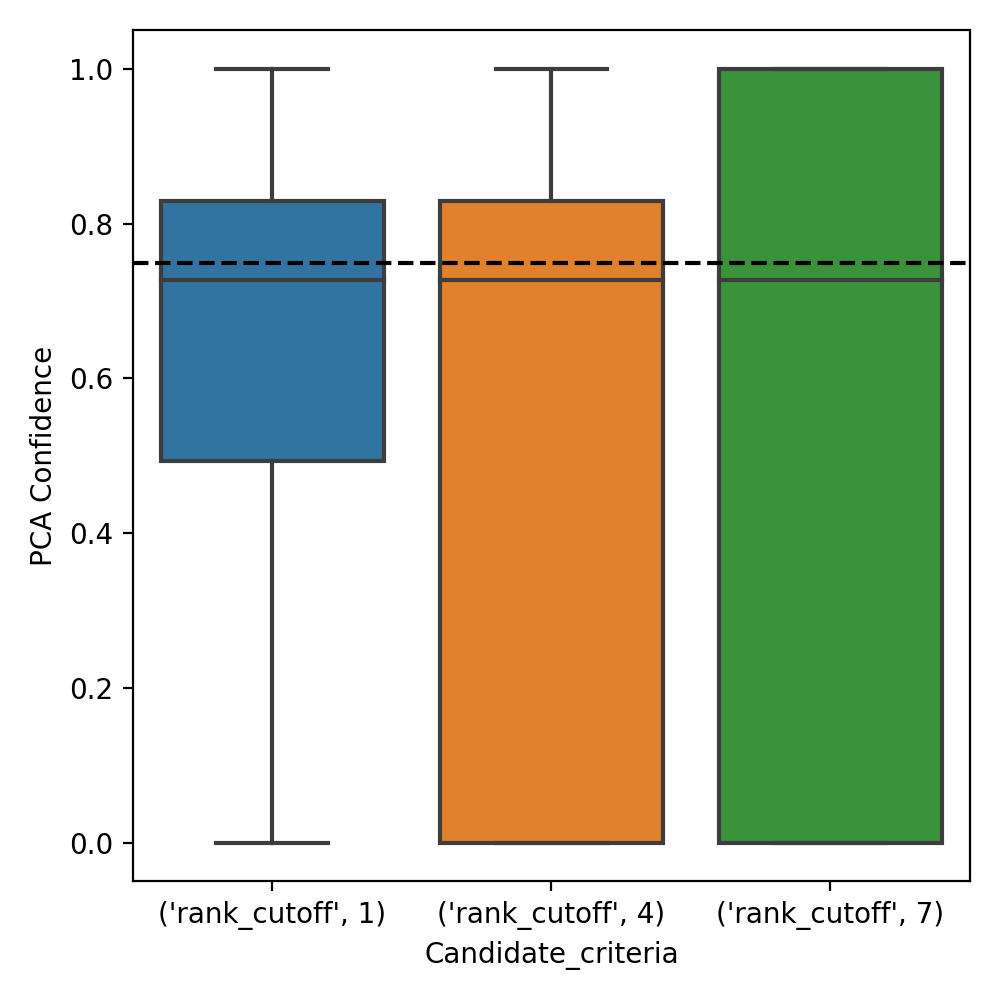
\includegraphics[width=1\linewidth]{figures/results/ranks/PCA-rank_wn18rr.png}
  \caption{Original WN18RR KG}
  \label{fig:PCA-rank_wn18rr_boxplot_sub}
\end{subfigure}%
\begin{subfigure}{.5\textwidth}
  \centering
  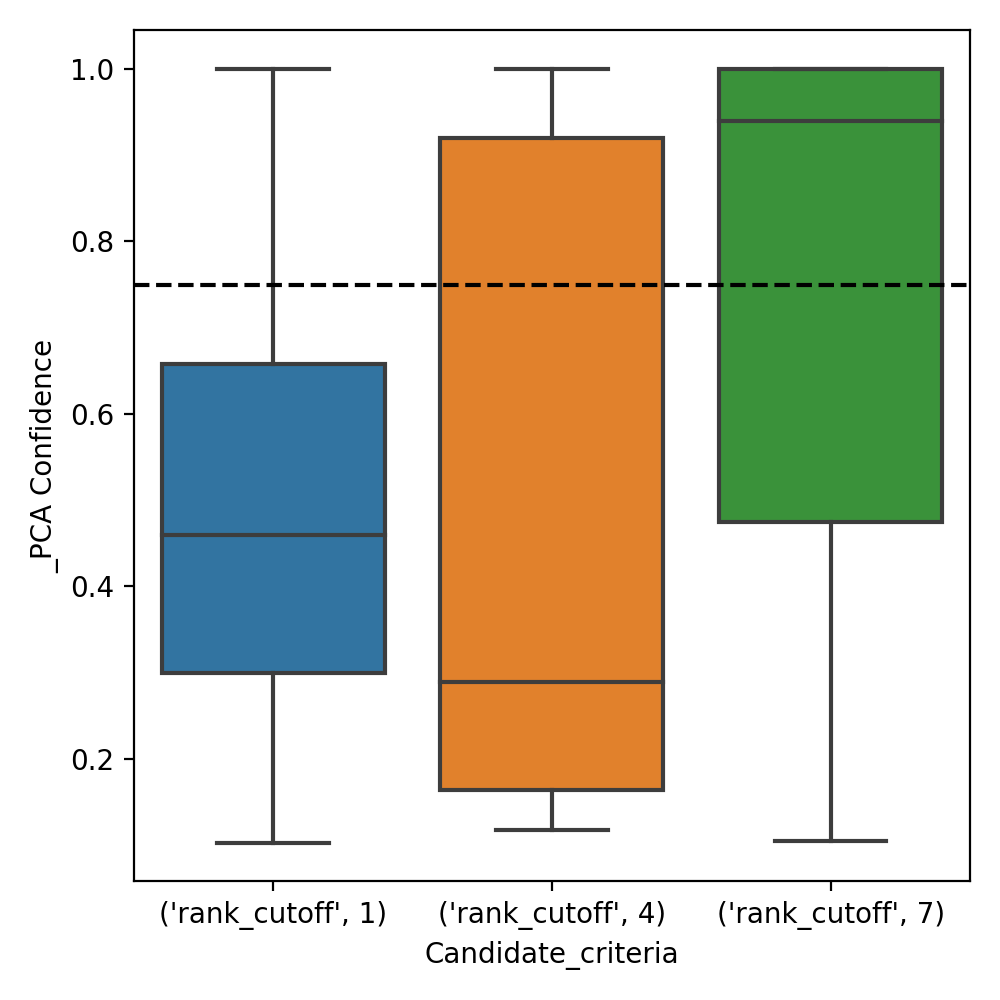
\includegraphics[width=1\linewidth]{figures/results/ranks/_PCA-rank_wn18rr.png}
  \caption{Extended WN18RR KG}
  \label{fig:_PCA_rank_wn18rr_boxplot_sub}
\end{subfigure}
\begin{subfigure}{.5\textwidth}
  \centering
  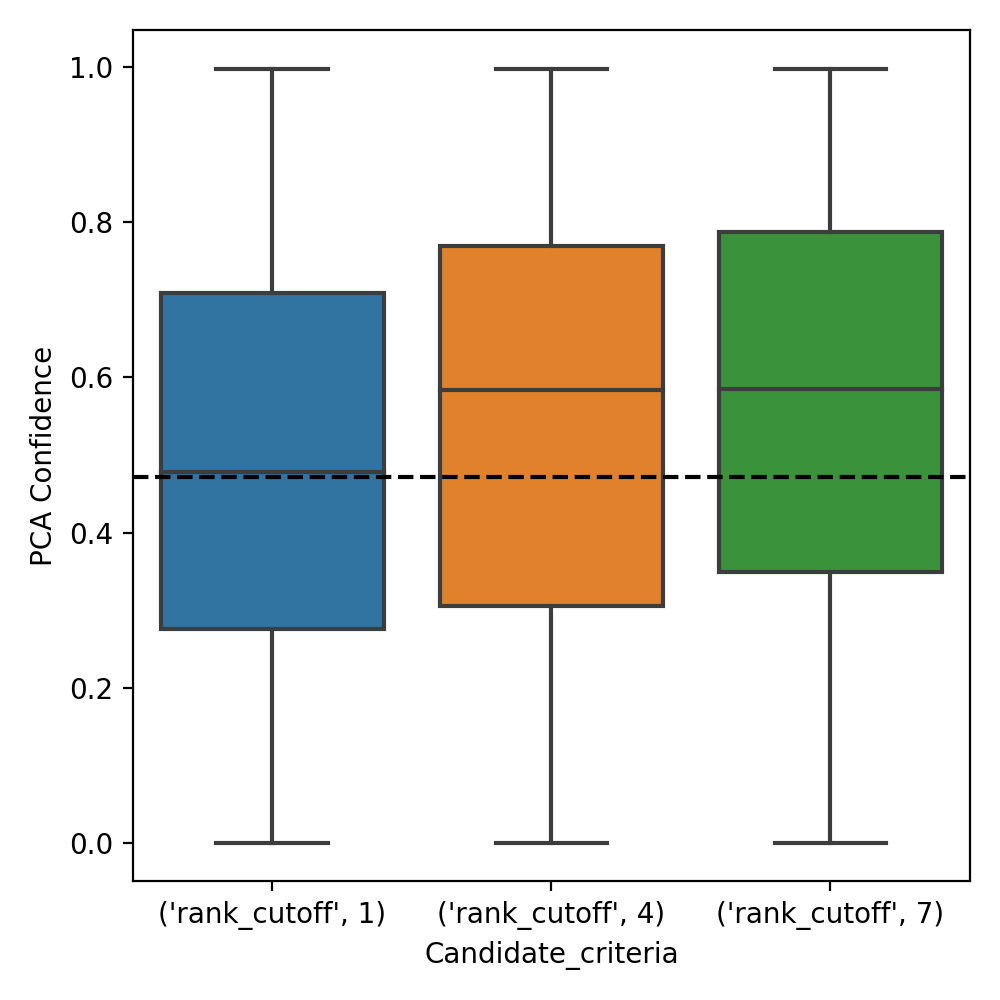
\includegraphics[width=1\linewidth]{figures/results/ranks/PCA-rank_family.png}
  \caption{Original family KG}
  \label{fig:models_rank_boxplot_sub}
\end{subfigure}%
\begin{subfigure}{.5\textwidth}
  \centering
  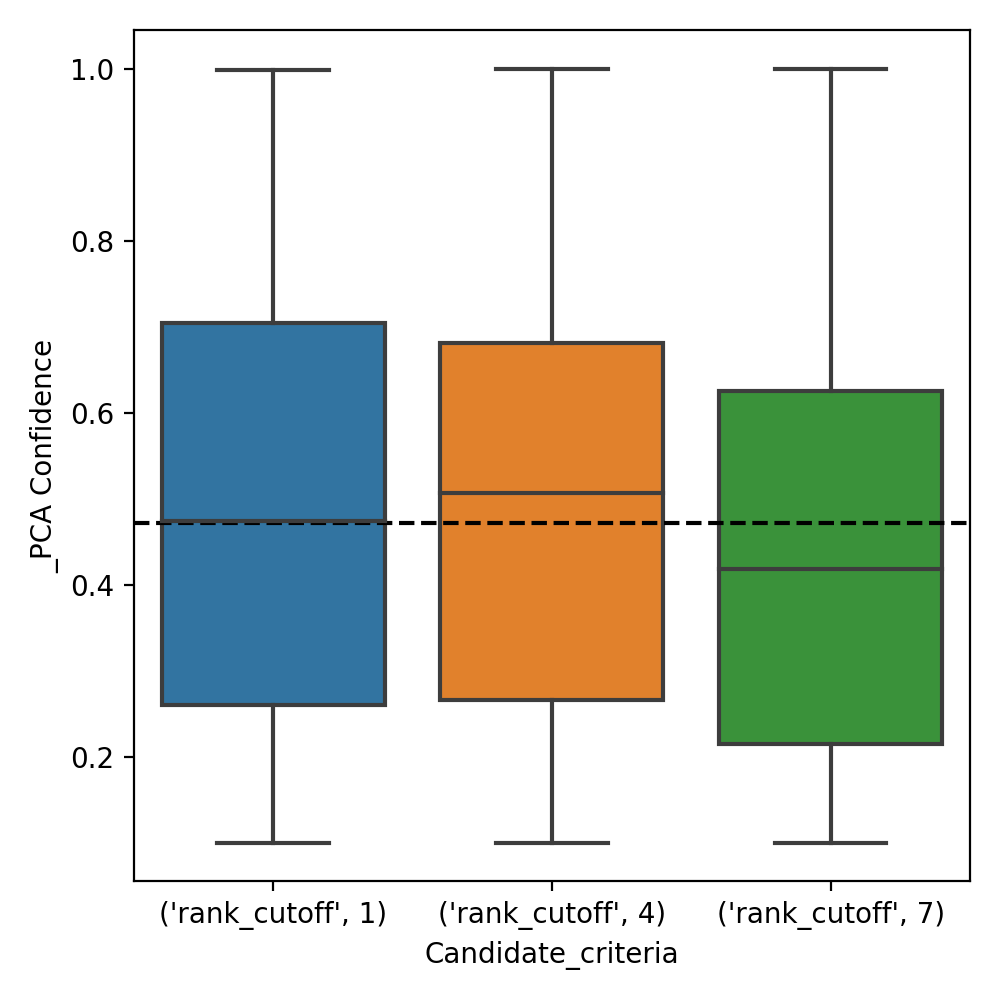
\includegraphics[width=1\linewidth]{figures/results/ranks/_PCA-rank_family.png}
  \caption{Extended family KG}
  \label{fig:_PCA_rank_family_boxplot_sub}
\end{subfigure}
\caption[Dist. of PCA conf. of rules over rank cutoff values]{Distribution of PCA confidence of mined rules over rank cutoff values. PCA confidence scores are calculated on the original KG (\ref{fig:PCA-rank_wn18rr_boxplot_sub}, \ref{fig:models_rank_boxplot_sub}) and the extended KG from which the rules are mined (\ref{fig:_PCA_rank_wn18rr_boxplot_sub}, \ref{fig:_PCA_rank_family_boxplot_sub}). A rule can be mined from multiple KGs, therefore this graph shows duplicates. The dashed line represents the median PCA confidence of the rules mined from the original KG.}
\label{fig:PCA_rank_boxplot}
\end{figure}


\begin{table}[htp]
\centering
\begin{tabular}{ccccccc}
\multicolumn{1}{c}{\multirow{2}{*}{\textbf{Rank cutoff}}} & \multicolumn{2}{c}{\textbf{Orig. rules}} & \multicolumn{2}{c}{\textbf{New Rules}}   & \multicolumn{2}{c}{\textbf{Orig. not found}} \\
\multicolumn{1}{c}{}                                      & Count & \multicolumn{1}{c|}{\% of mined} & Count & \multicolumn{1}{c|}{\% of mined} & Count            & \% of original            \\ \hline
\multicolumn{1}{l|}{1}                                    & 10    & \multicolumn{1}{c|}{50\%}        & 10    & \multicolumn{1}{c|}{50\%}        & 0                & 0 \%                        \\
\multicolumn{1}{l|}{4}                                    & 4     & \multicolumn{1}{c|}{27\%}        & 11    & \multicolumn{1}{c|}{73\%}        & 6                & 60\%                      \\
\multicolumn{1}{l|}{7}                                    & 3     & \multicolumn{1}{c|}{20\%}        & 12    & \multicolumn{1}{c|}{80\%}        & 7                & 70\%                     
\end{tabular}
\caption[Dist. of rules over rank cutoff - WN18RR KG.]{Distribution of all the rules mined over rank cutoff values. KG: WN18RR.}
\label{Tab:table_rules_ranks_wn18rr}
\end{table}


\begin{table}[htp]
\centering
\begin{tabular}{ccccccc}
\multirow{2}{*}{\textbf{Rank cutoff}} & \multicolumn{2}{c}{\textbf{Orig. rules}} & \multicolumn{2}{c}{\textbf{New Rules}}   & \multicolumn{2}{c}{\textbf{Orig. not found}} \\
                                      & Count & \multicolumn{1}{c|}{\% of mined} & Count & \multicolumn{1}{c|}{\% of mined} & Count            & \% of original            \\ \hline
\multicolumn{1}{c|}{1}                & 94    & \multicolumn{1}{c|}{90\%}        & 11    & \multicolumn{1}{c|}{10\%}        & 0                & 0 \%                        \\
\multicolumn{1}{c|}{4}                & 90    & \multicolumn{1}{c|}{51\%}        & 85    & \multicolumn{1}{c|}{49\%}        & 4                & 4\%                       \\
\multicolumn{1}{c|}{7}                & 88    & \multicolumn{1}{c|}{45\%}        & 108   & \multicolumn{1}{c|}{55\%}        & 6                & 6\%                      
\end{tabular}
\caption[Dist. of rules over rank cutoff - family KG.]{Distribution of all the rules mined over rank cutoff values. KG: family.}
\label{Tab:table_rules_ranks_family}
\end{table}
    
\subsection{Summary of effect of parameters}
The three parameters for KG extension were shown to have a varying degree of influence. All entity selection strategies, apart from \textit{most likely}, performed equally well. This was consistent with the assumption of the authors of AmpliGraph, being that the most frequent entities are less likely to have missing facts \cite{ampligraph}. Of the KG embedding models, TransE led to a substantially greater number of new rules being mined compared to the other models, but these rules had very low PCA confidence when calculated over the original dataset. ComplEx and DistMult performed similarly in regard to PCA confidence, with slightly more new rules being mined with DistMult due to the model giving candidate triples a higher score than ComplEx did. The rank cutoff value gave expected results, where a value that accepted more new candidate triples led to more new rules being minded. When calculated over the original KG, the PCA confidence in rules did not significantly vary among the rank cutoff values. 

\newpage
\section{Rule comparison}
In the WN18RR dataset there was one rule, 
\[derivationally\_related\_form(y, x) \Rightarrow derivationally\_related\_form(x, y)\]
which was mined in all 48 KG extensions. It has PCA confidence of 1, meaning that there are no data points in WN18RR that do not follow the rule. In table \ref{wn18rr_original_rules_table_PCA} all original rules sorted by their PCA Confidence are listed. How often these rules were mined from KG extensions is also listed under the "Frequencies" column. Using Spearman's rank correlation coefficient there was found a correlation coefficient of 0.65 with $p$-value 0.04. These values are positively correlated with the PCA confidence, meaning that as the PCA confidence increases, the frequency also increases. From the family KG, 94 original rules were mined, and the corresponding table \ref{family_original_rules_table_PCA} is listed in the appendix. For these rules the PCA confidence and frequencies were also positively correlated with correlation coefficient 0.86 and $p$-value $5.85e^{-29}$. The rule mined the least number of times is
\[father(x,z) \wedge sibling(z, y) \Rightarrow relative(x, y)\]
which only was mined in 10 out of the 48 extensions. Consistently with the correlation between PCA confidence and mining frequency this is the rule with the second lowest PCA confidence. The table \ref{family_original_rules_table_PCA} also shows us that all rules that had the \textit{relative} predicate were not mined for all 48 extensions, and all with different predicates in the antecedent were mined from all extensions. This could be due to the simple fact that \textit{relative} is the least frequently used relation in the KG, leading to less supporting data points and correspondingly lower PCA confidence.



\label{Rule_comparison}
\begin{table}[htbp]
\begin{tabular}{lrr}
\toprule
                                                                                                      Rule &  Frequencies &  PCA Confidence \\
\midrule
                            DRF(y, x)   $\Rightarrow$ DRF(x, y) &           48 &        1.000000 \\
          IH(x, z) $\wedge$ SDTO(z, y)   $\Rightarrow$ SDTO(x, y) &           24 &        0.886525 \\
                   hypernym(x, z) $\wedge$ SDTO(z, y)   $\Rightarrow$ SDTO(x, y) &           36 &        0.828871 \\
                   has\_part(x, z) $\wedge$ SDTO(z, y)   $\Rightarrow$ SDTO(x, y) &           24 &        0.809524 \\
                   has\_part(z, x) $\wedge$ SDTO(z, y)   $\Rightarrow$ SDTO(x, y) &           24 &        0.771739 \\
                   hypernym(z, x) $\wedge$ SDTO(z, y)   $\Rightarrow$ SDTO(x, y) &           34 &        0.726667 \\
                                      has\_part(x, z) $\wedge$ IH(y, z)   $\Rightarrow$ has\_part(x, y) &           19 &        0.532544 \\
DRF(x, z) $\wedge$ SDTO(z, y)   $\Rightarrow$ SDTO(x, y) &           24 &        0.492857 \\
DRF(z, x) $\wedge$ SDTO(z, y)   $\Rightarrow$ SDTO(x, y) &           24 &        0.492857 \\
                                               has\_part(x, z) $\wedge$ hypernym(y, z)   $\Rightarrow$ has\_part(x, y) &           21 &        0.104016 \\
\bottomrule
\end{tabular}
\caption[Rules mined from the original WN18RR KG]{Rules mined from the original WN18RR KG, with their corresponding PCA confidences and how many times they were mined from the 48 extensions. DRF = ``\textit{derivationally related form}", STDO = ``\textit{synset domain topic of}" and IH = ``\textit{instance hypernym}".}
\label{wn18rr_original_rules_table_PCA}
\end{table}



\subsection{PCA distribution}
For both the WN18RR and family KG the PCA confidence of the original rules is relatively spread out. A few rules have a PCA confidence of 1 or close to 1, and none have PCA confidence below 0.1. This makes sense, because this would imply the absence of supporting datapoints and thus AMIE3 would never mine the rule. The majority of new rules on the other hand \textit{do} however have a PCA confidence of 0. This means that most, if not all, the support for new rules lies in the extension of the KG. If all sets of supporting datapoints are dependent on the extension, then when PCA confidence is measured on the original KG this new rule would get a PCA confidence score of 0. If one looks closely at figure \ref{fig:PCA_rule_dist_new_original_family_sub} one can see that two new rules do have PCA confidence above 0.2. These were however also rejected by AMIE3 because the PCA body size (the number of instances of that rule) is so small that the PCA confidence calculated is not very reliable.

When plotting the PCA confidence of new rules calculated over the KGs from which they were mined, the new rules become somewhat more evenly distributed along the PCA confidence interval. Figures \ref{fig:_PCA_rule_dist_new_original_wn18rr_sub} and \ref{fig:_PCA_rule_dist_new_original_family_sub} shows this, where the PCA confidence of the new rules here is not calculated over the original KG, rather the KG from which they were mined that gave them the best PCA confidence score. This method was chosen to highlight the extent to which the extensions changes the PCA confidence of new rules.

\begin{figure}[htbp]
\centering
\begin{subfigure}{.49\textwidth}
  \centering
    \includesvg[inkscapelatex=false,width=1\textwidth,keepaspectratio]{figures/results/rule_comparison/PCA_rule_dist_new_original_wn18rr.svg}
    \caption{WN18RR - Original KG}
  \label{fig:PCA_rule_dist_new_original_wn18rr_sub}
\end{subfigure}
\begin{subfigure}{.49\textwidth}
  \centering
    \includesvg[inkscapelatex=false,width=1\textwidth,keepaspectratio]{figures/results/rule_comparison/PCA_rule_dist_new_original_family.svg}
    \caption{Family - Original KG}
  \label{fig:PCA_rule_dist_new_original_family_sub}
\end{subfigure}
\begin{subfigure}{.49\textwidth}
  \centering
    \includesvg[inkscapelatex=false,width=1\textwidth,keepaspectratio]{figures/results/rule_comparison/_PCA_rule_dist_new_original_wn18rr.svg}
    \caption{WN18RR - Extended KG}
  \label{fig:_PCA_rule_dist_new_original_wn18rr_sub}
\end{subfigure}%
\begin{subfigure}{.49\textwidth}
  \centering
    \includesvg[inkscapelatex=false,width=1\textwidth,keepaspectratio]{figures/results/rule_comparison/_PCA_rule_dist_new_original_family.svg}
    \caption{Family - Extended KG}
  \label{fig:_PCA_rule_dist_new_original_family_sub}
\end{subfigure}
\caption[PCA conf. dist. of new and original rules.]{Distribution of PCA confidence of original rules and new rules. In subfigures \ref{fig:PCA_rule_dist_new_original_wn18rr_sub} and \ref{fig:PCA_rule_dist_new_original_family_sub} the PCA confidence is calculated over the original KG. For subfigures \ref{fig:_PCA_rule_dist_new_original_wn18rr_sub} and \ref{fig:_PCA_rule_dist_new_original_family_sub} the PCA confidence is the best score calculated over the extended KG from which the new rules was mined. The PCA confidence of original rules is always calculated over the original KG.}
\label{fig:PCA_rule_dist_new_original}
\end{figure}


\section{Summary of findings}
\label{results_summary}
We restate the central questions for the experiment posed at the beginning of this chapter. These questions were:
\begin{enumerate}
    \item Does adding new plausible facts lead to new rules being mined? 
    \item How does the PCA confidence of these rules compare to the rules mined from the original KG?
    \item Can the rules mined from the original KG also be mined after the KG is extended?
\end{enumerate}

Questions 1 is the simplest, and our experiment has clearly shown that, yes, adding new plausible facts does result in new rules being mined. Examples of rules that were mined after extending the KGs are:
                            \begin{center}
                            relative(z, x) $\wedge$ relative(y, z) $\Rightarrow$ relative(x, y) \\
                          father(x, y) $\wedge$ mother(x, y) $\Rightarrow$ child(x, y) \\
                            father(y, z) $\wedge$ mother(x, z) $\Rightarrow$ sibling(x, y) \\
                            relative(z, y) $\wedge$ spouse(x, z) $\Rightarrow$ relative(x, y) \\
                             relative(x, z) $\wedge$ relative(y, z) $\Rightarrow$ relative(x, y) \\
                            father(x, z) $\wedge$ mother(y, z) $\Rightarrow$ sibling(x, y) \\
                             \end{center}
At close inspection these rules are relatively poor, and as seen in figure \ref{fig:PCA_rule_dist_new_original} the PCA confidence of new rules was most often zero or close to zero when calculated over the original KG. However, when measured on the extended KGs from which they were mined, the scores were significantly better and had similar distributions to the original rules, which answers question 2. In regard to question 3, a strong correlation was found between the PCA confidence of original rules and how often the rule was mined from extended KGs. The higher the PCA confidence, the more likely the rule will be mined from the extended KG.

%In regard to the influence the parameters had on the outcomes of the experiment, the chosen KG embedding model clearly had the most influence. TransE performed ever worse than the baseline model, resulting in unusually many nonsense rules being mined in comparison to the embedding models. ComplEx and DistMult resulted in fewer rules with higher PCA confidence, with ComplEx being more conservative in the ranking of candidate triples. All entity selection methods gave similar resluts, apart from \textit{most frequent} which resulted in 

\section{Limitations of experiment}
\label{experiment_limitations}
The experiment has many limitations, most related to computational restrictions. When generating candidates, for example, the optimal approach would be to generate all possible candidates, and evaluate them all. This is simply not possible due to computational limitations. As mentioned in section \ref{canidate_triple_generation}, there are more intelligent strategies for entity selection, but these were also too computationally intensive to take into use. A larger and better set of candidate triples would substantially strengthen the conclusions about KG embedding model and rank cutoff values when evaluating parameters in the KG extension process. This is because when only a small fraction of the possible candidates are ranked by models, we get an incomplete picture of the model's behaviour.

The hyperparameter search for the KG embedding models could also be improved upon with greater computational resources, but it is not as influential as increasing the candidate set size and quality. This is due to the fact the random search has been shown to measure well against grid search \cite{li2017hyperband}, so the effect on the performance of the model is likely to be minimal.